\clearpage
\section{Implemented Thread network}

\subsection{Thread network topology}
With the three Blind Access Points and the Border Router I have created a test of my own Thread network. I did this in an apartment with a floor space of 40\,\si{\metre\squared} and placed the four devices on four points in the house. After successfully connecting each device, the resulting topology was as shown in Figure \ref{fig:topology}. It can be clearly seen that three of the four devices were in the Router role and one was in the End Device (Child) role. This is observed because OpenThread tries to keep the number of routers participating in the whole Thread network between 16 and 23 devices. This topology has evolved because, at the time the image was taken, one of the FTD devices had not yet been able to designate itself as a router. During testing, the devices were in stable connection with each other and all devices were available in the network.
\begin{figure}[!htb]
    \centering
    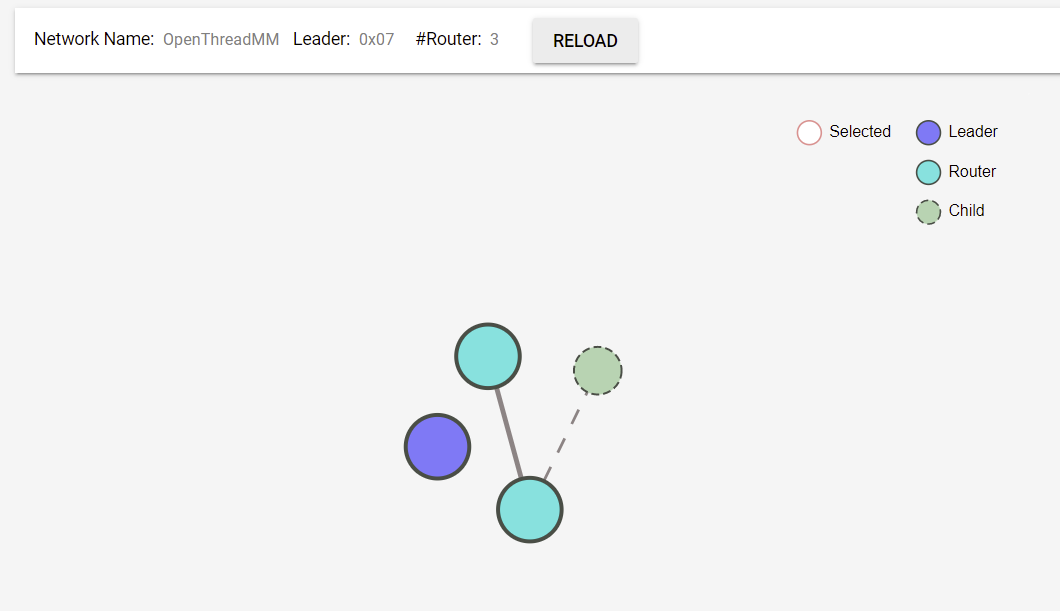
\includegraphics[width=\textwidth]{img/topologia.png}
    \caption{My Thread network topology}
    \label{fig:topology}
\end{figure}

\pagebreak
\subsection{Border Router in operation}
\begin{figure}[!htb]
    \centering
    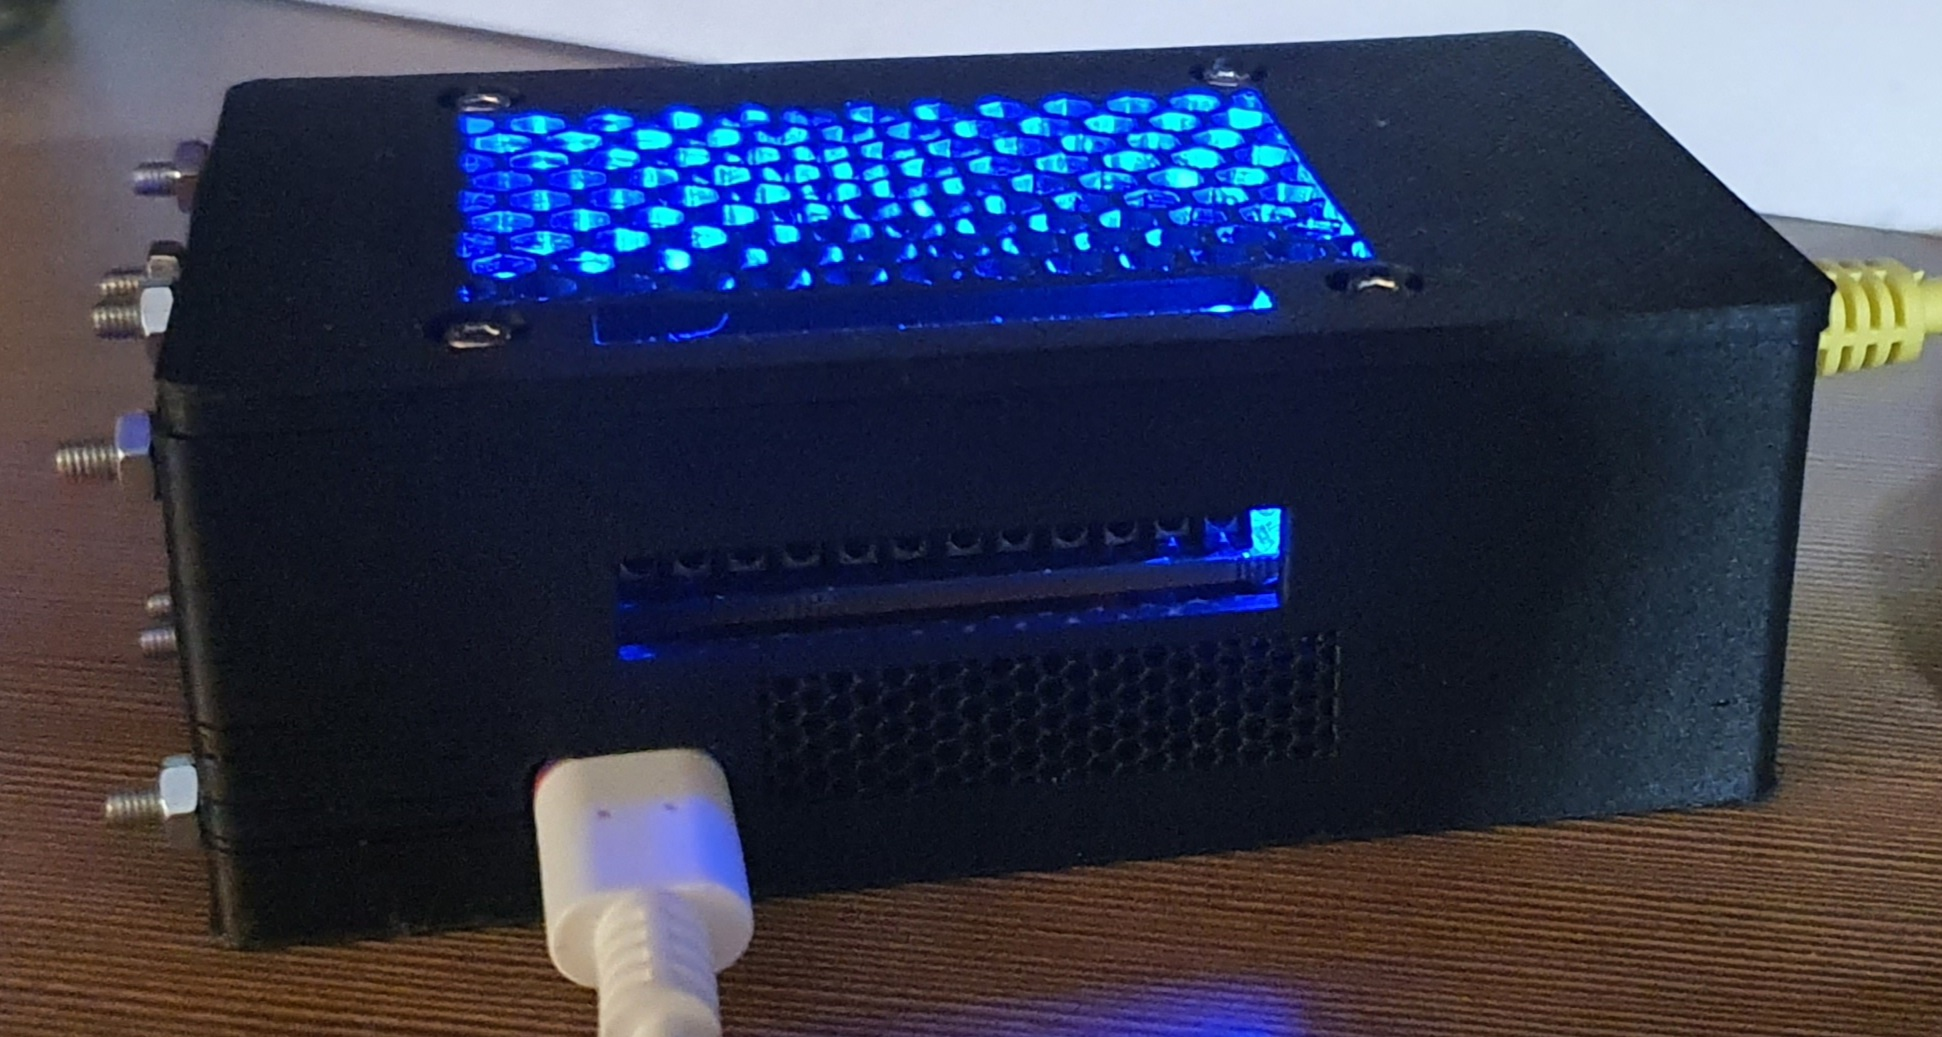
\includegraphics[width=\textwidth]{img/valosborderrouter.jpg}
    \caption{Assembled Border Router}
    \label{fig:realborderrouter}
\end{figure}

\subsection{The completed Blind Access Point}
\begin{figure}[!htb]
    \centering
    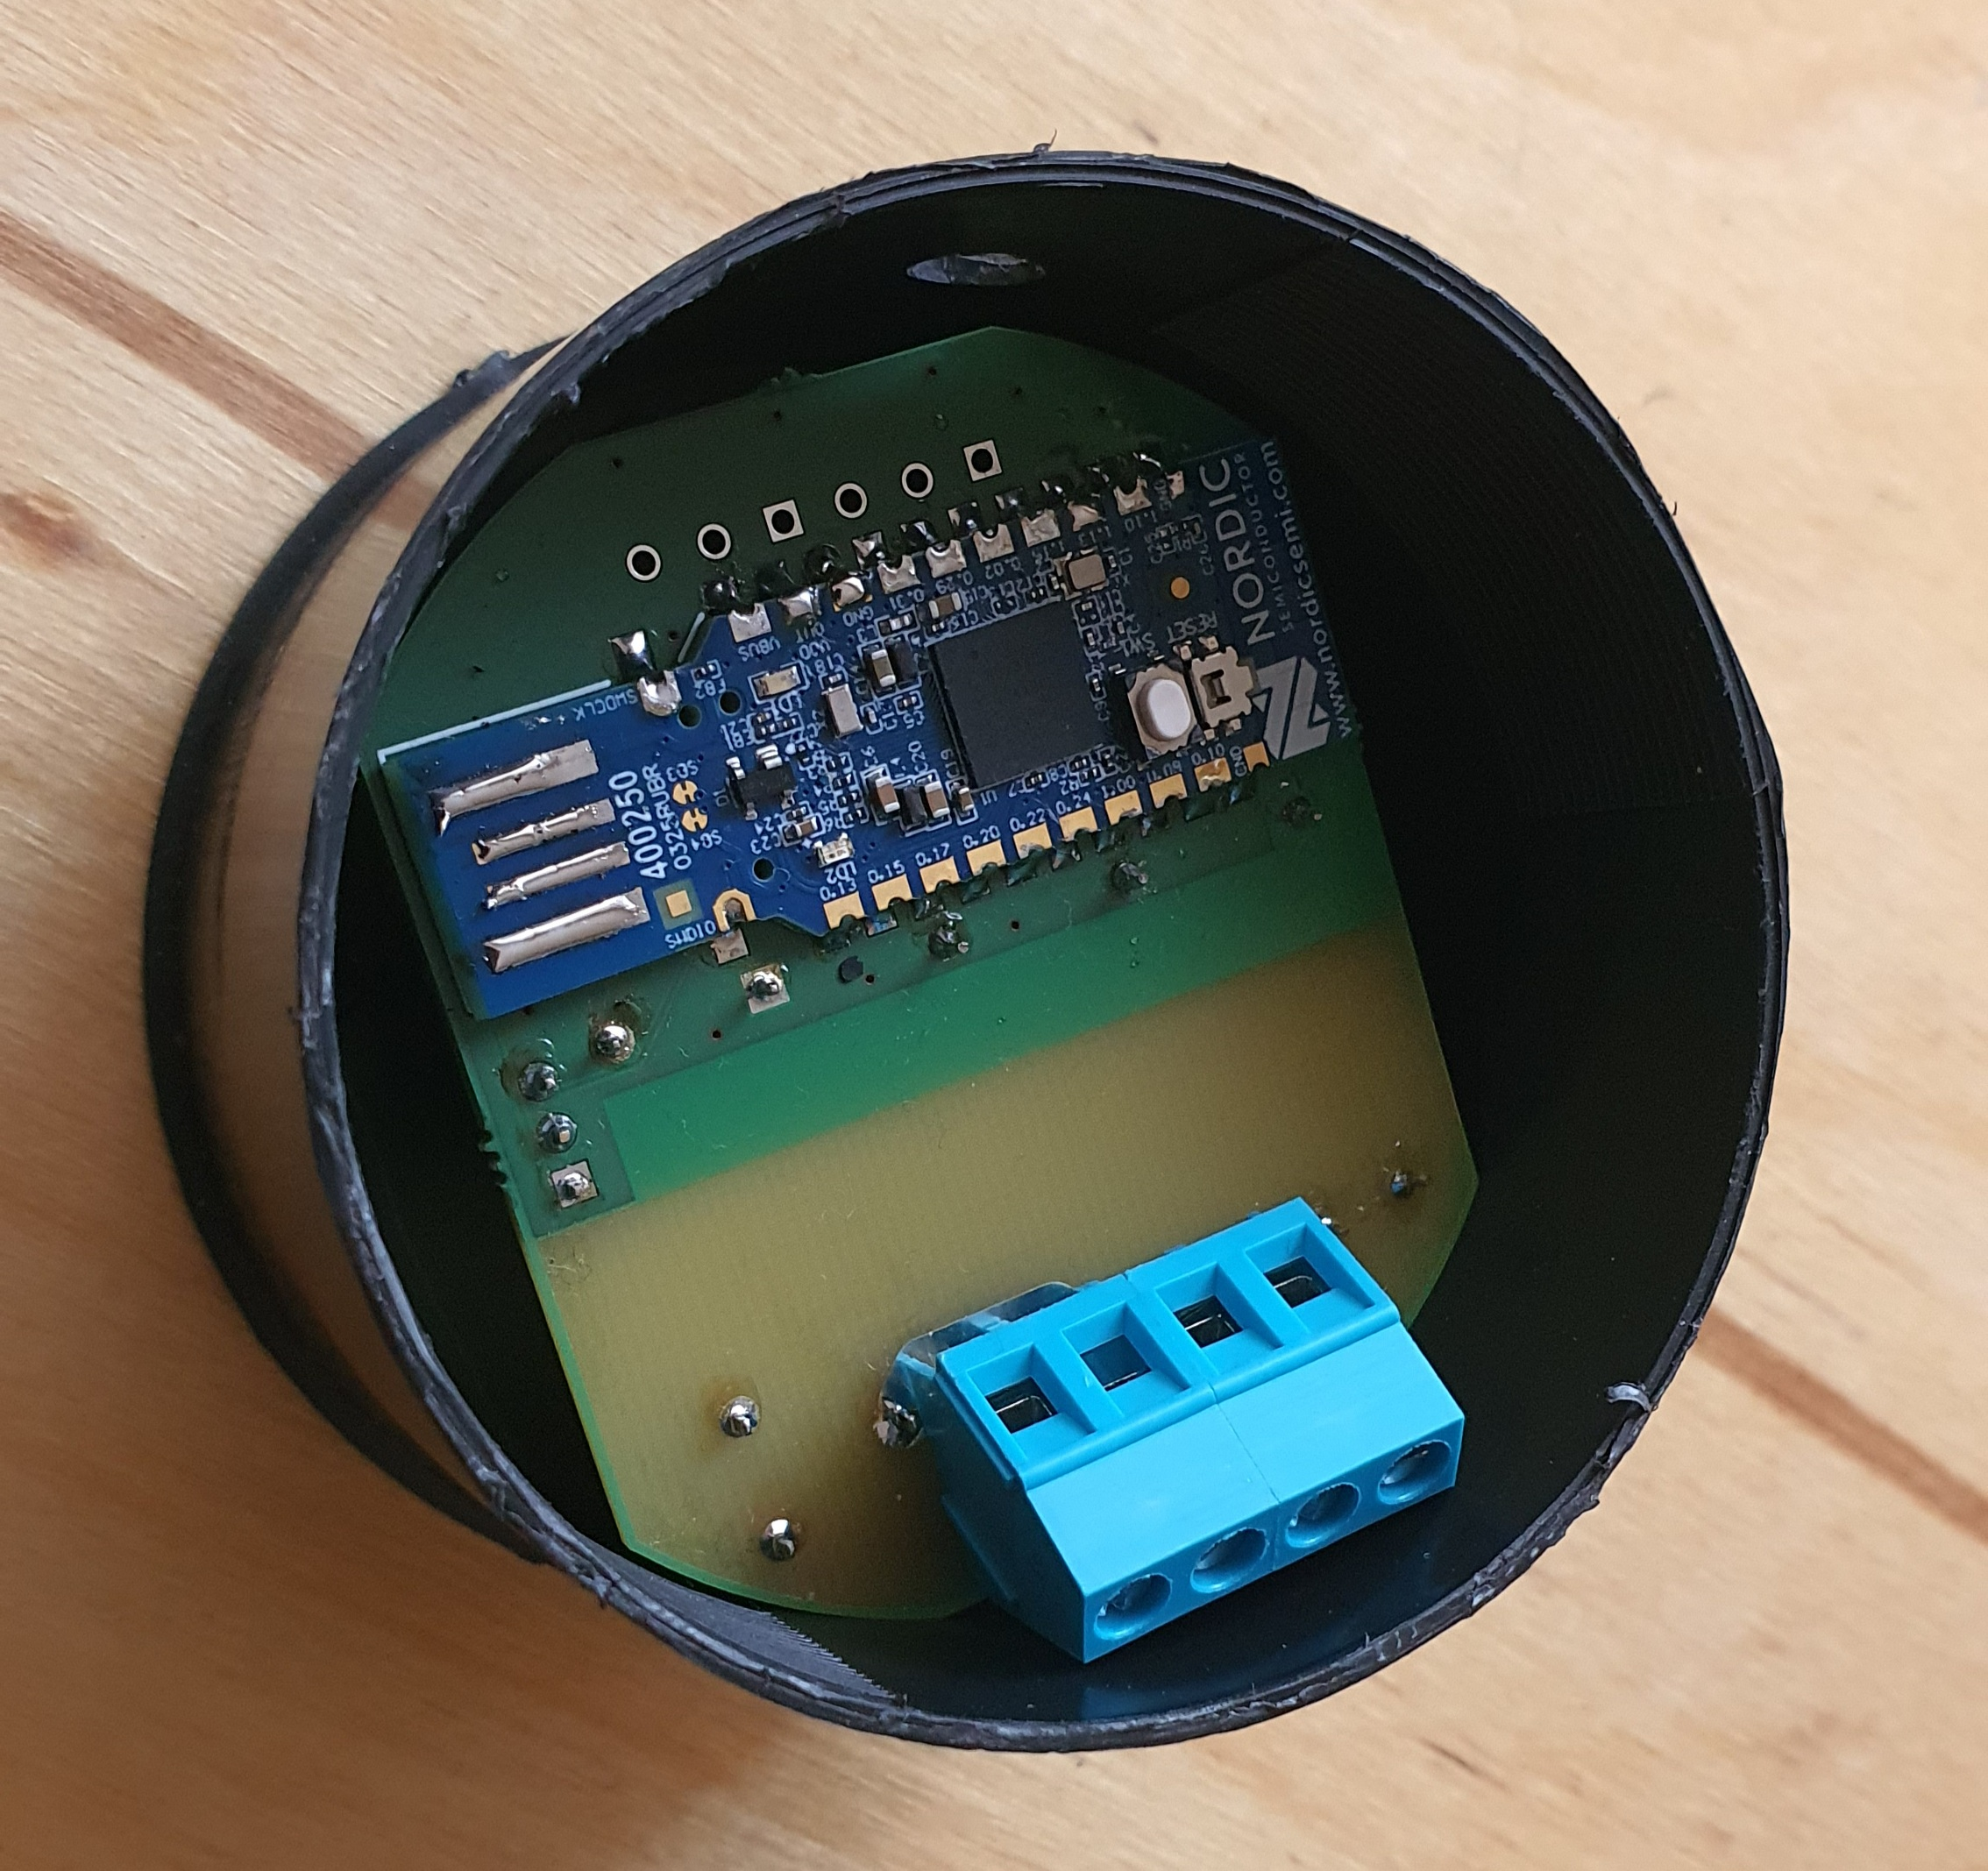
\includegraphics[scale=0.1]{img/realblindaccesspoint.jpg}
    \caption{Assembled Blind Access Point in the assembly box}
    \label{fig:realblindaccesspoint}
\end{figure}

\subsection{The completed Minimal Sensor Node}
\begin{figure}[!htb]
    \centering
    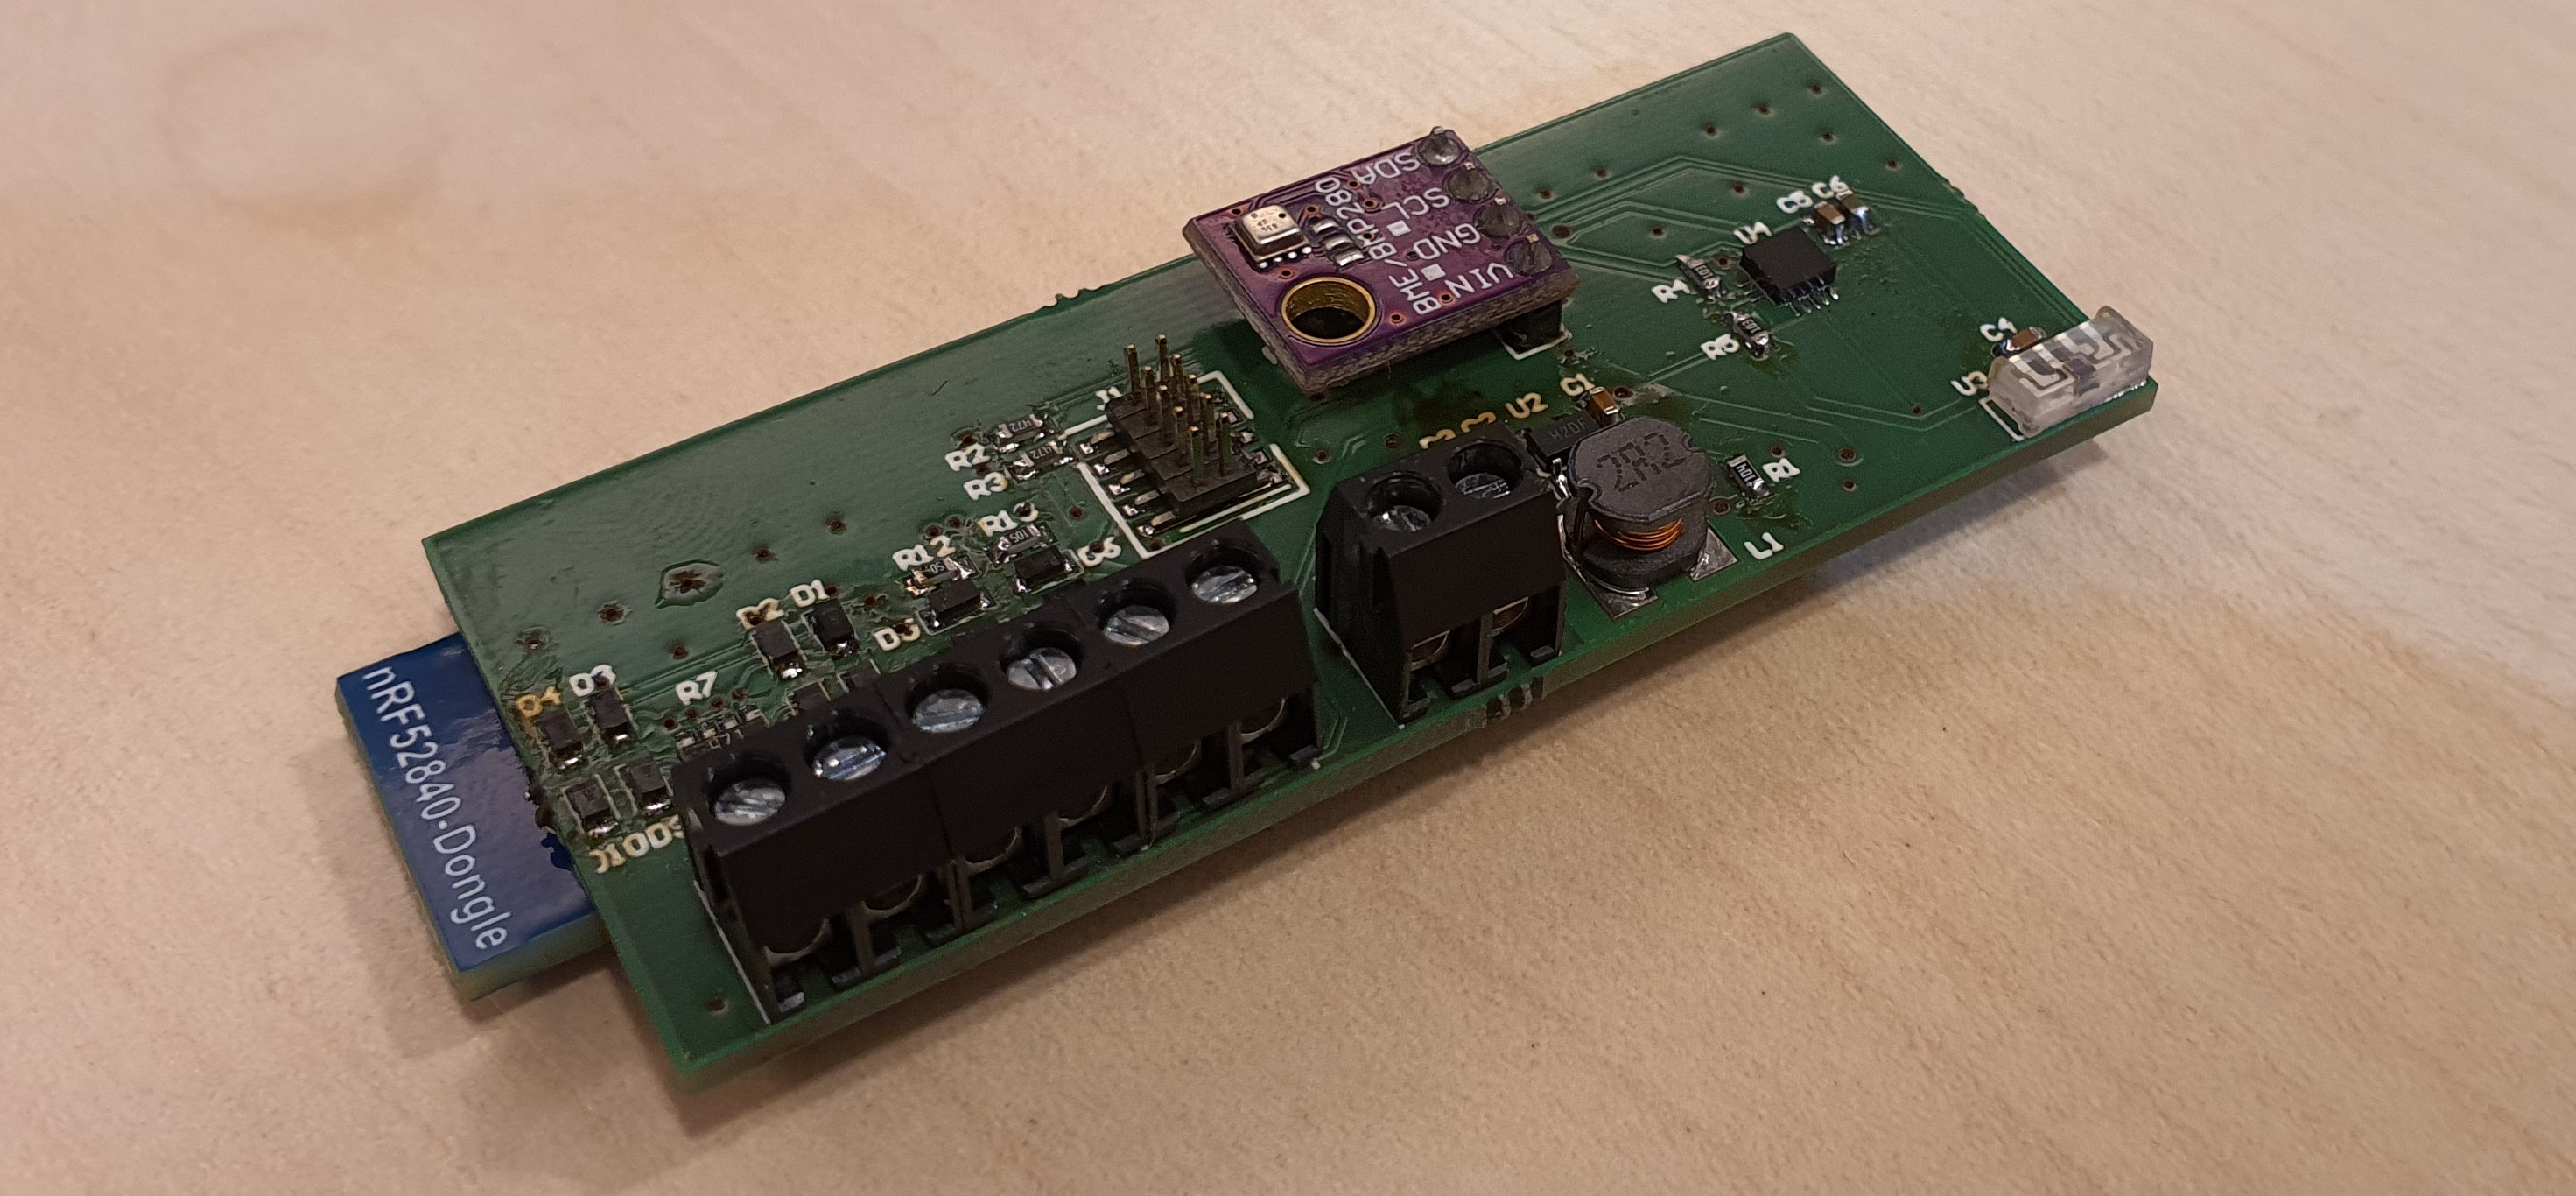
\includegraphics[width=\textwidth]{img/minimalupperside.jpg}
    \caption{Completed Minimal Sensor Node upper side}
    \label{fig:realminimalup}
\end{figure}
\begin{figure}[!htb]
    \centering
    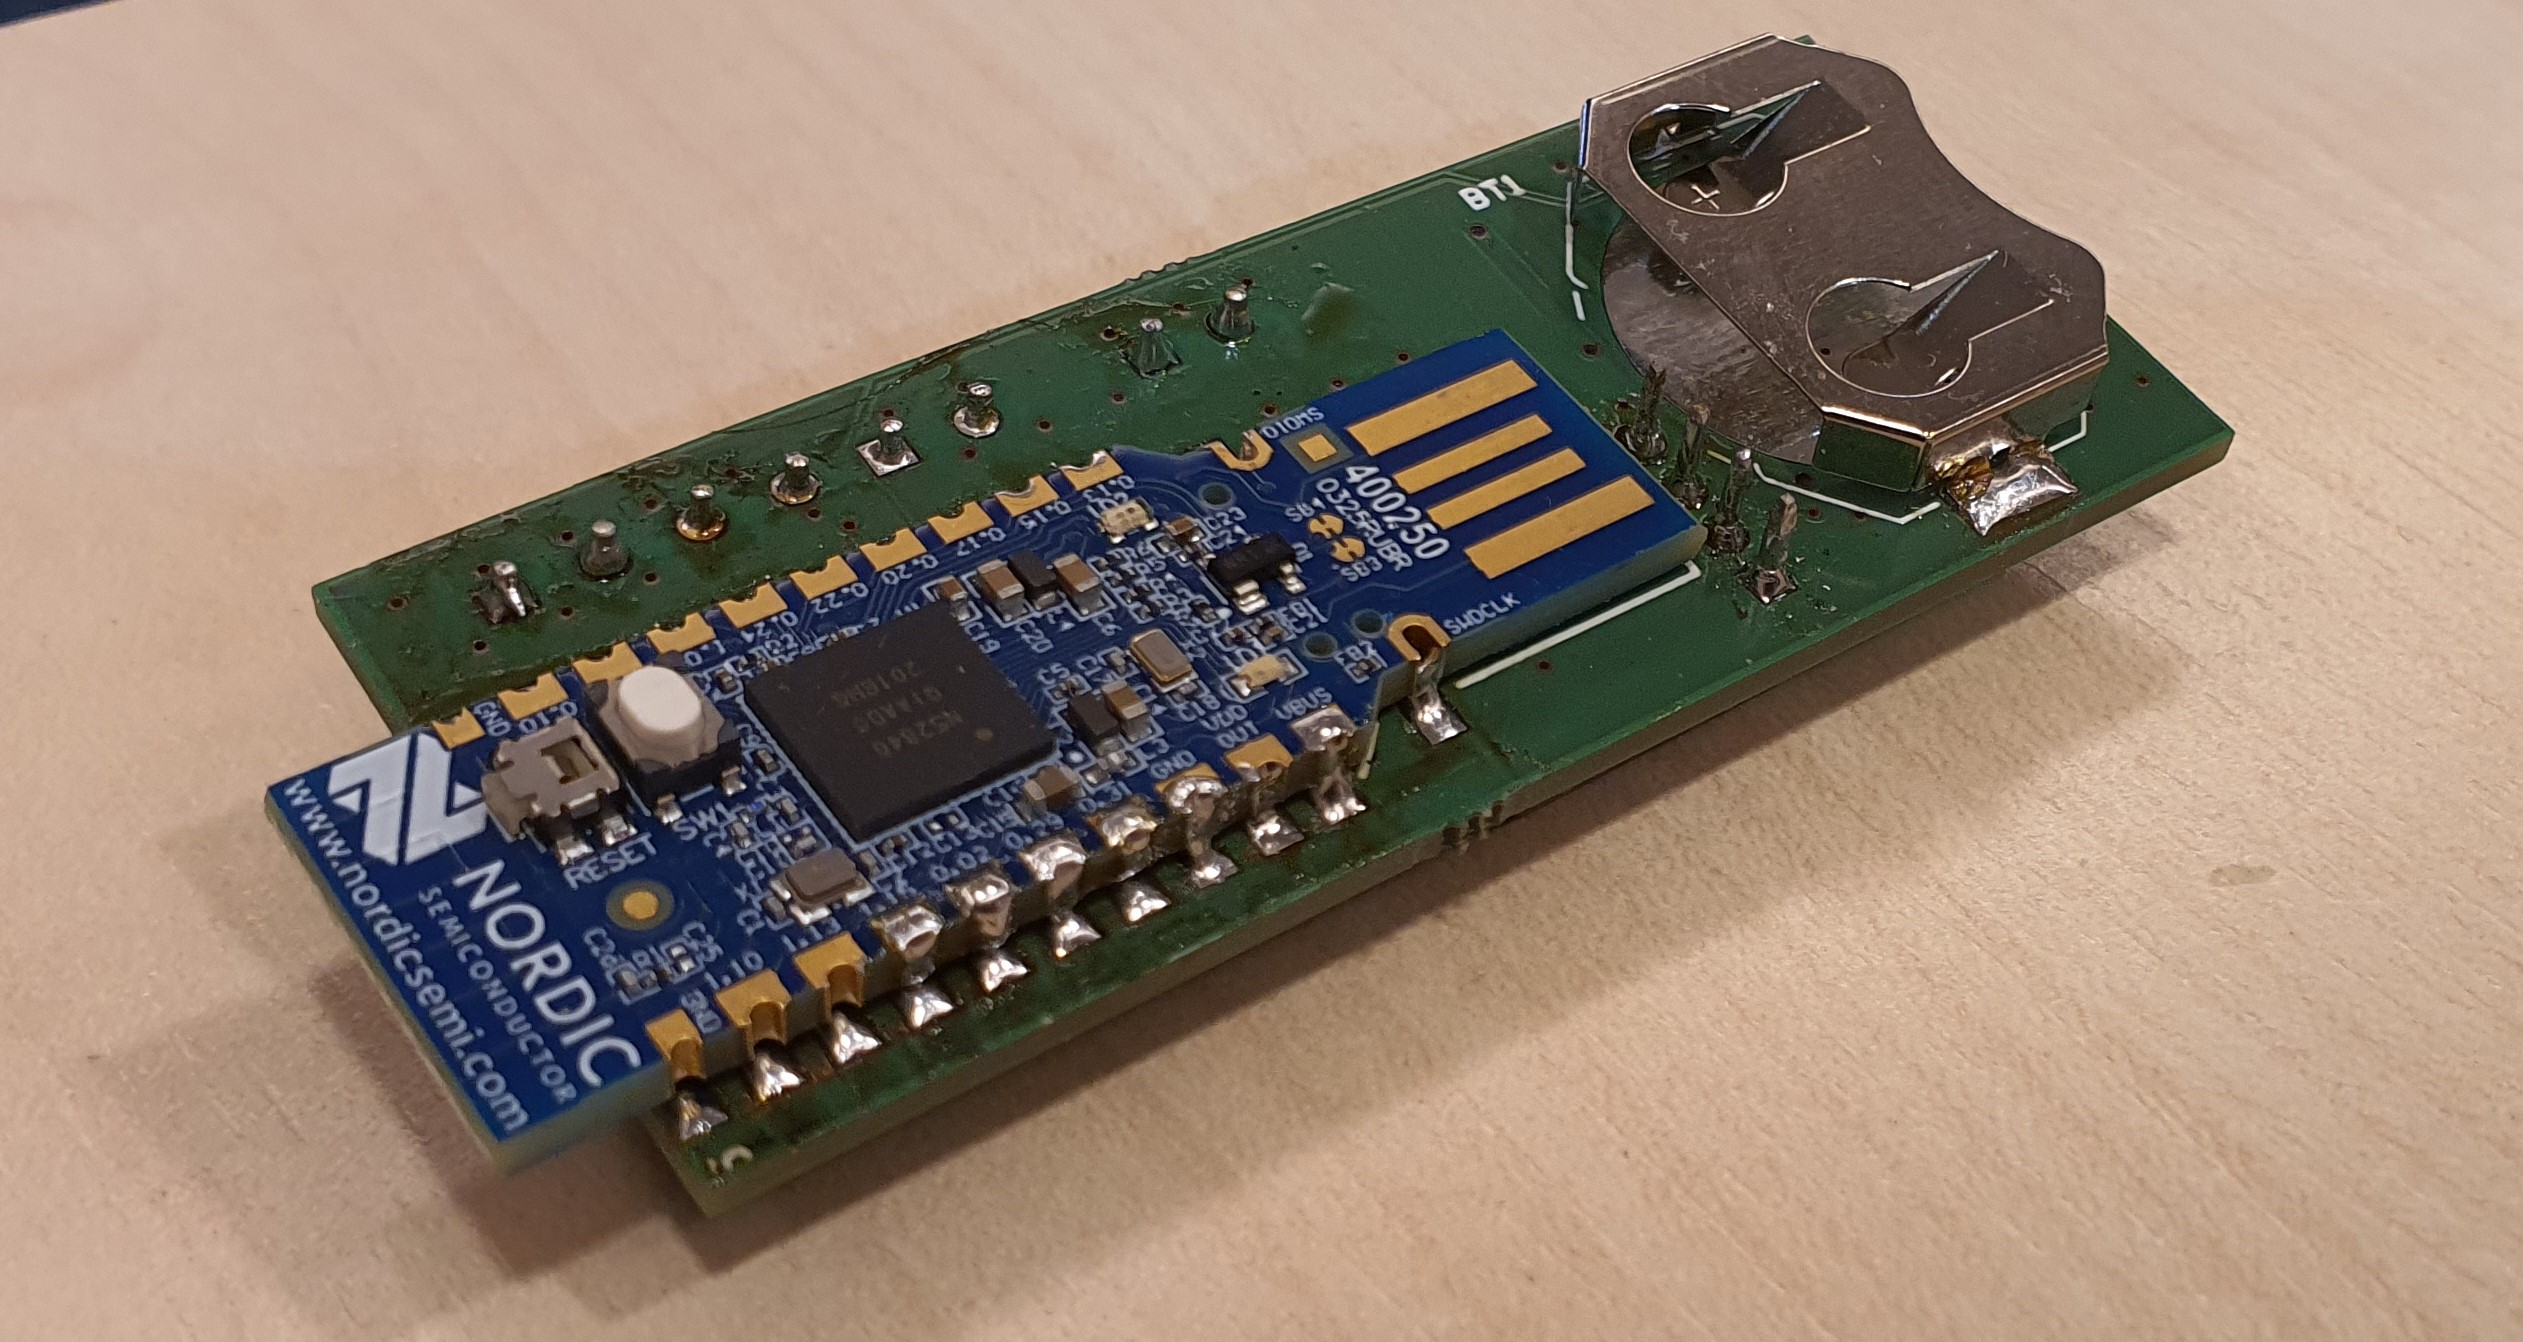
\includegraphics[width=\textwidth]{img/minimaldownside.jpg}
    \caption{Completed Minimal Sensor Node lower side}
    \label{fig:realminimaldown}
\end{figure}


\subsection{Insight}
The use cases I have presented, represent only a small part of the feasible devices. Large US companies like Apple and Google have also released several devices that support the Thread protocol. Such devices include the Apple HomePod mini and the Google Nest Hub Max. For those interested, a detailed list of Thread-certified devices is available at \href{https://www.threadgroup.org/What-is-Thread/Thread-Benefits}{Thread Group}\cite{devices}. 